The solver \texttt{phaseFieldFoam} has already been validated for various problems multiple times. Simulations with a wedge were also conducted with adaptive mesh refinement in \cite{holzinger2021DirectNumericalSimulation}. Simulations of capillaries or parallel plates were carried out in Hagg \cite{hagg2019DirekteNumerischeSimulation} and by Cai et al. \cite{cai2015NumericalSimulationWetting}. Samkhaniani et al. \cite{samkhaniani2021BouncingDropImpingement} simulated a bouncing droplet on a hydrophobic surface. Many other interesting and essential simulations and validations have been conducted with \texttt{phaseFieldFoam} \cite{bodziony2023StressfulWayDroplets,yinDirectNumericalSimulation,worner2021SpreadingReboundDynamics,bagheriInterfacialRelaxationCrucial2022}, whose individual mention would go beyond the scope of this work.
Since the solver has been validated in many places, only a Laplace test is conducted in this work. With Equation \ref{eq: YoungLaplaceEQ}, the pressure difference can be calculated for a settling radius of the simulation's interface and compared with the theoretical value. For this comparison, the radius of the interface in the simulation must be known. Assuming that the circle's center lies on the axis of rotation, the radius can be calculated using
\begin{equation}
    r_{\mathrm{S}} = \frac{R^2}{2h}+\frac{h}{2}
\end{equation}
\begin{figure}[h]
    \centering
    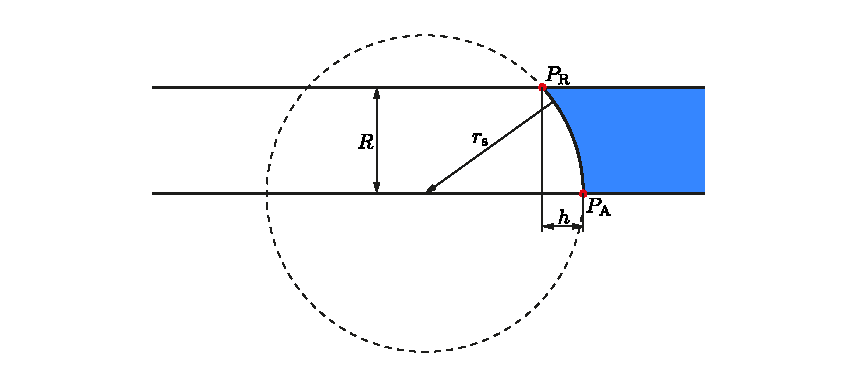
\includegraphics[width=.95\textwidth]{Pictures/RadiusCalc.pdf}
    \caption{Schematic of the capillary with relevant dimensions for the calculation of the radius}
    \label{fig: RadiusCalc}
\end{figure}

Figure \ref*{fig: RadiusCalc} shows the geometry of the capillary with the relevant dimensions. The points $P_{\mathrm{R}}$ and $P_{\mathrm{A}}$ are the intersection points of the interface with the capillary wall and the axis of rotation. If these points are known, the height $h$ of the spherical segment can be calculated, and thus the sphere's radius $r_{\mathrm{S}}$ with the already known capillary radius $R$. The dashed line is intended to clarify that the sphere's radius does not necessarily have to correspond to that of the capillary.
